\documentclass{article}

% for images: png, pdf, etc
\usepackage{graphicx}

% for nice table formatting, i.e. /toprule, /midrule, etc
\usepackage{booktabs}

% to allow for \verb++ declarations in captions.
\usepackage{cprotect}

% for nice source code syntax highlighting, also provides Listing env
%\usepackage{minted}

% for nice units
\usepackage{siunitx}

% for less margin space
\usepackage{fullpage}

% for nice todo notes
\usepackage{todonotes}

\author{Jason K. Moore and Antonie van den Bogert}

\title{Direct Control Identification in Human Gait}

\date{}

\begin{document}

\maketitle

\section*{TODO}

\listoftodos

\section*{Introduction}
%
Recent research and commercial activity indicate that gait-related powered
prosthetics will play an important role in both assisting humans with
disabilities and enhancing the abities of able bodied. These devices include a
variety of sensors and actuators than can be coupled to a control system to
provide acutated gait assistance. However, for example, the available
lightweight lower extremity exoskeletons lack gait that resembles an
able-bodied human. It is difficult to design a controller from first principles
for this very non-linear system. Although work based on \cite{Geyer2010} are
giving promising results in simulated musculoskeletal systems \cite{Wang2010,
Geitenbeek2014}. Even though constraining the controller to rudimentary models
of the muscoulo skeleteal system is fruitful, we are curious if more generic
black box control models can reveal more robust controllers. To improve the
gait of powered prosthetics, our intent is to identify a simple, linear
controller from a large set of data collected from able-bodied subjects being
perturbed by random longitudinal forces.

There are other researchers thinking along these lines. Elliot Rouse identified
the parameters of a linear model of the ankle's passive and active stiffness
and damping by perturbing around 400 stance phases of the gait cycle and
fitting a model with linear least squares. \cite{Wang2013} are able to predict
the foot placement with a simple lienar model derived from kinematic data.
%
\section*{Methods}
%
\subsection*{Experiments}
%
We make use of a subset of the gait data reported in \cite{Moore2015} and refer
the reader to that publication for more details about the experiments and data.
The subset of the data includes a large number of gait cycles for 11 subjects
subjects walking at three nominal speeds on a treadmill with and without
pseudo-random longitudinal perturbations, i.e fluctuations in the belt speed.
The subject metadata parameters are given in Table~\ref{tab:subjects}.
%
\begin{table}
  \cprotect\caption{Information about the 11 study participants. The final
    three columns provide the trial numbers associated with each nominal
    treadmill speed. The measured mass is computed from the mean total vertical
    ground reaction force just after the calibration pose event. Generated by
    \verb|src/subject_table.py|.}
  \centering
  \begin{tabular}{rlrrrrrr}
\toprule
 Id &  Gender &  Age [yr] & Height [m] &                     Mass [kg] & 0.8 m/s & 1.2 m/s & 1.6 m/s \\
\midrule
    &         &           &            &                               &         &         &         \\
  3 &  female &        32 &       1.62 &      $54\pm2$ &      46 &      47 &      48 \\
  5 &    male &        23 &       1.73 &  $71.2\pm0.9$ &      32 &      31 &      33 \\
  6 &    male &        26 &       1.77 &  $86.8\pm0.6$ &      40 &      41 &      42 \\
  7 &  female &        29 &       1.72 &  $64.5\pm0.8$ &      16 &      17 &      18 \\
  8 &    male &        20 &       1.57 &  $74.9\pm0.9$ &      19 &      20 &      21 \\
 10 &    male &        19 &       1.77 &      $92\pm2$ &      61 &      62 &      63 \\
 12 &    male &        22 &       1.85 &  $74.2\pm0.5$ &      49 &      50 &      51 \\
 13 &  female &        21 &       1.70 &      $58\pm2$ &      55 &      56 &      57 \\
 15 &    male &        22 &       1.83 &  $80.5\pm0.8$ &      67 &      68 &      69 \\
 16 &  female &        28 &       1.69 &  $56.2\pm0.6$ &      76 &      77 &      78 \\
 17 &    male &        23 &       1.86 &  $88.3\pm0.8$ &      73 &      74 &      75 \\
\bottomrule
\end{tabular}

  \label{tab:subjects}
\end{table}

\subsection*{Data Preprocessing}
%
The ``raw'' data provided by \cite{Moore2015} consists of 100~\si{\hertz} time
series of marker and ground reaction loads in addition to event time
identifiers. We make use of an open source software package,
GaitAnalysisToolKit, to process the data. The processing follows these steps:
%
\begin{enumerate}
  \item Identify missing marker data.
  \item Replace missing marker data with linearly interpolated values.
  \item Filter all signals with a forward/backward 2nd order low pass
    Butterworth filter with a cutoff frequency of 6~\si{\hertz}.
  \item Section the trials into unperturbed and perturbed sections based on the
    event times.
  \item Compute the planar inverse dynamics for the lower body: right and left
    ankle, knee, hip joint angles, joint angular rates, and joint torques.
  \item Identify the heelstrike times based on the vertical ground reaction
    force.
  \item Segment the time series into gait cycles based on the right foot's
    heelstrikes.
  \item Interpolate the time series in each gait cycle to a specific number of
    data points so all gait cycles have the same number of samples.
  \item Throw out any outlier gait cycles that were not properly identified due
    to abnormal ground reaction force measurements.
\end{enumerate}

After the initial processing above, the data is stored in three dimensional
arrays M x N x ?, where M is the number of gait cycles, N is the number of time
instances in the gait cycle, and ? are the number of time series.
Figure~\ref{fig:angle-torque-comparison} shows the mean and standard deviation
of across the gait cycles for selected time series for both unperturbed and
perturbed walking. Furthermore, Figure~\ref{fig:gait-cycle-stats-comparison}
compares several gait statistics of interest for unperturbed and perturbed
walking. These two figures are intended to show that there is variation in the
subject's motion that is a direct result of the longitudinal perturbations.
%
\begin{figure}
  \centering
  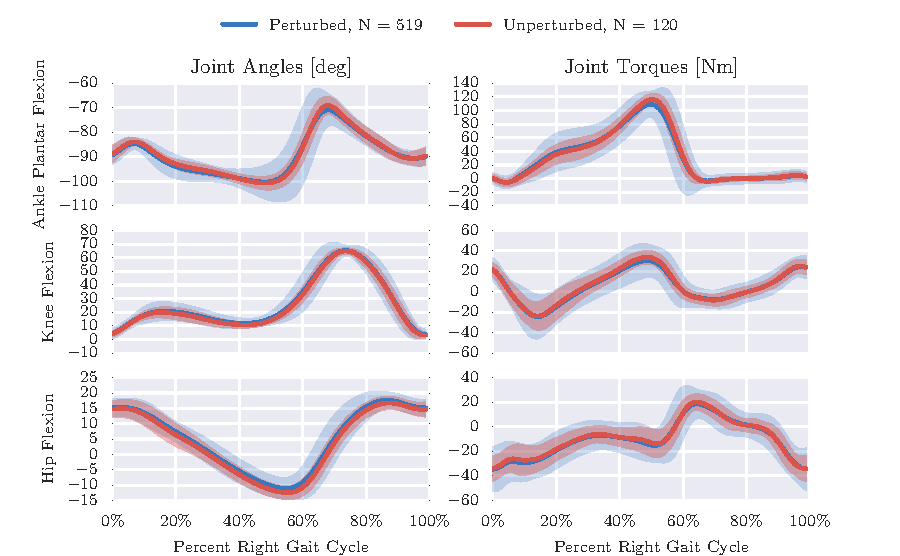
\includegraphics{figures/unperturbed-perturbed-comparison.pdf}
  \cprotect\caption{Right leg mean and $3\sigma$ (shaded) joint angles and
    torques from both unperturbed (red) and perturbed (blue) gait cycles
    from trial 20. We define the nominal configuration, i.e. all joint angles
    equal to zero, such that the vectors from the shoulder to the hip, the hip
    to the knee, the knee to the ankle, and the heel to the toe are all aligned.
    Produced by \verb|src/unperturbed_perturbed_comparison.py|.}
  \label{fig:angle-torque-comparison}
\end{figure}
%
\begin{figure}
  \centering
  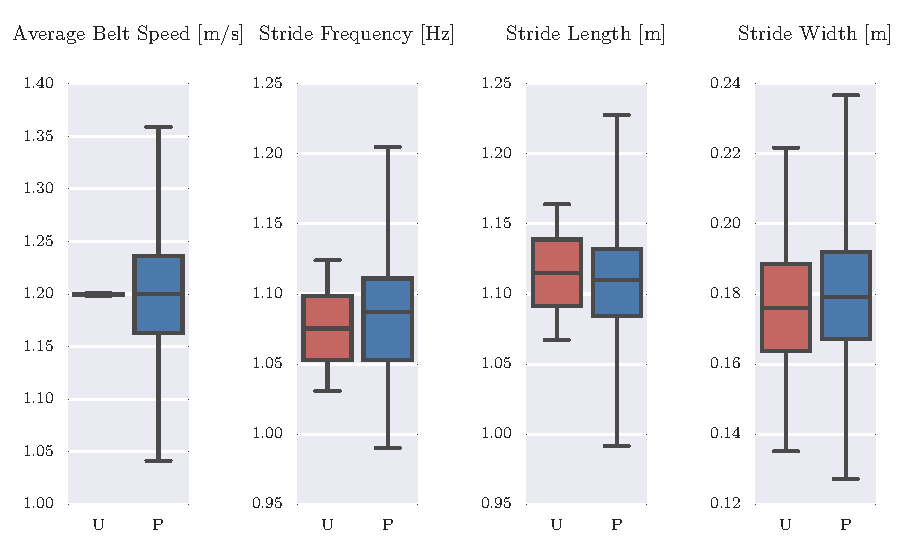
\includegraphics{figures/unperturbed-perturbed-boxplot-comparison.pdf}
  % NOTE : Make sure to update these values (120, 519) if anything in the
  % script changes.
  \cprotect\caption{Box plots of the average belt speed, stride frequency,
    stride length, and stride width which compare 120 unperturbed (U: red) and
    519 perturbed (P: blue) gait cycles. The median is given with the box
    bounding the first and third quartiles and the whiskers bound the range of
    the data. Produced by \verb|src/unperturbed_perturbed_comparison.py|.}
  \label{fig:gait-cycle-stats-comparison}
\end{figure}

\subsection*{Controller}
\label{sec:controller}
%
We assume a black box~\footnote{black box in the system identification sense,
i.e. there are parameters in the model} control structure for the closed loop
system, Figure~\ref{fig:controller}. We first assume there is an unknown
non-linear plant, i.e. the open loop musculoskeletal system and treadmill, that
has an uknown time varying state. This plant can be perturbed by an external
exogenous input $w(t)$, in our case by varying belt speed, and is also driven
by joint torques $\mathbf{m}(t)$. An unknown sensor model generates feedback
signals, $\mathbf{s}(t)$, that are compared to a nomimal gait phase dependent
reference trajectory $\mathbf{s}_0(\varphi)$ that describes the gait phase
varying state for cyclic gait when no feedback is necessary. The error in these
sensors are fed into the controller which generate corrective joint torques
that are added to the nomimal gait phase dependent joint torques
$\mathbf{m}_0(\varphi)$ that correspond to the nominal trajectories,
$\mathbf{s}_0(\varphi)$. We then assume that when the actual state deviates
from the nominal state trajectory that the controller computes additive joint
torques based on the state tractory error to compensate for variation in gait
away from the nomimal.

The controller is designated as a gait phase scheduled gain matrix,
$\mathbf{K}(\varphi)$ that relates the error in the state trajectories to the
additive joint torques. The controller structure bounded by the box in
Figure~\ref{fig:controller} can be described by the following algebraic
equation.
%
\begin{equation}
  \mathbf{m}(t) = \mathbf{m}_0(\varphi) + \mathbf{K}(\varphi) [\mathbf{s}_0(\varphi) - \mathbf{s}(t)]
  \label{eq:controller}
\end{equation}
%
\begin{figure}
  \centering
  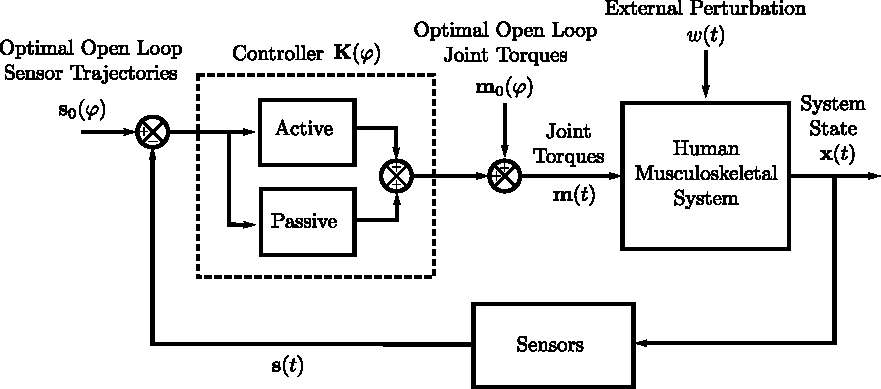
\includegraphics{figures/control-system.pdf}
  \caption{The controller block diagram}
  \label{fig:controller}
\end{figure}

It is important to note that this control structure will effectively lump the
passive control gains with the active ones in addition to any other unmodeled
effects. This is desirable for our intentions, as we are only concerned with
mapping this identified controller to that of powered prosthetic device and it
is thuse unnessary to distinguish between these.

\subsection*{Direct Identification}
%
We employ a direct identification approach to find the optimal parameters for
the control structure described in Section~\ref{sec:controller}. We are aware
that direct identifcation has its drawbacks. It is well known that process
noise due to unmodeled affects in the identification model will bias the
results towards the inverse of the plant if the external perturbations are not
sufficiently large enough~\cite{Ljung1999,Kearney1990,Kooij2005}. Determining
if the perturbations are of large enough size is difficult because the process
noise is generally unknown.

\todo[inline]{I need to explain why we think our perturbations may be large
  enough in magnitude. The problem is that we get similiar identification
  results from both unpertrubed and perturbed data. THis can mean one of two
  things: (1) the person perturbs themselves enough and the identification is
  correct either way or (2) our perturbations are not enough, i.e. we'd get
  different results by perturbing more. The only thing that I can think of here
  is to show the necessary perturbation level for the quiet standing case and
  then say that we have similar magnitudes.}

We reformulate Equation~\ref{eq:controller} to make it amenable to linear
identifaction. The equation can be rewritten so that is linear in the gains and
a new term $\mathbf{m}^*$.
%
\begin{equation}
  \mathbf{m}(t) = \mathbf{m}^*(\varphi) - \mathbf{K}(\varphi) \mathbf{s}(t)
  \label{eq:linear-form}
\end{equation}
%
where
%
\begin{equation}
  \mathbf{m}^*(\varphi) = \mathbf{m}_0(\varphi) + \mathbf{K}(\varphi) \mathbf{s}_0(\varphi)
\end{equation}

Assuming that we can collect noisy measurements of $\mathbf{m}(t)$
and $\mathbf{s}(t)$, $\mathbf{m}^*(\varphi)$ and $\mathbf{K}(\varphi)$ are
identified simply by using linear least squares to regress the data. Given $m$
gait cycles with $n$ time steps in each gait cycle with $q$ controls and $p$
sensors there are $nq(p + 1)$ unknowns and $mnq$ equations so we need at least
$p + 1$ gait cycles to solve for the unknowns.

Details of coercing Equation~\ref{eq:linear-form} into the canonical form,
$\mathbf{Ax}=\mathbf{b}$ can be found in the supplementary IPython notebook
\verb|form_linear_system.ipynb|.

We compute the scheduled gains and $\mathbf{m}^*$ for both the unperturbed and
perturbed gait cycles for each trial. Three quarters of the data from each
series of gait cycles are used to compute the unknowns and the model is
validated against the remaining one quarter of the data. We compute the
percentatge of variance accounted for by the model with respect to the
validation data set to gauage how well the model predicts.

\begin{equation}
  \textrm{VAF} = 1 - \frac{||\mathbf{m}_p - \mathbf{m}_m||}
    {||\mathbf{m}_m - \bar{\mathbf{m}}_m||}
  \label{eq:vaf}
\end{equation}

\section*{Results}
%
The formulation above allows one to choose a variety of combinations of
potential sensor, $\mathbf{s}(t)$, and control, $\mathbf{m}(t)$, signals to
generate a controller.

\begin{description}
  \item[Joint Isolated Control] The torque generated by a joint is only
    affected by the sensors that give information about that joint.
\end{description}

\subsection*{Example Result}
%
The example data shown here was collected from a single subject (age: 29, mass:
63 kg, height: 172 cm) walking on an instrumented treadmill (V-Gait, Motek
Medical). The subject was longitudinally perturbed using random white noise
with 10\% std around a nominal 1.2 m/s belt speed. Data was recorded for 8
minutes at 100 Hz, which included approximately 500 steps of walking. Ankle
plantarflexion, knee flexion, and hip flexion angles, rates, and moments were
computed using 2D inverse dynamics.
%
\begin{figure}
  \begin{center}
    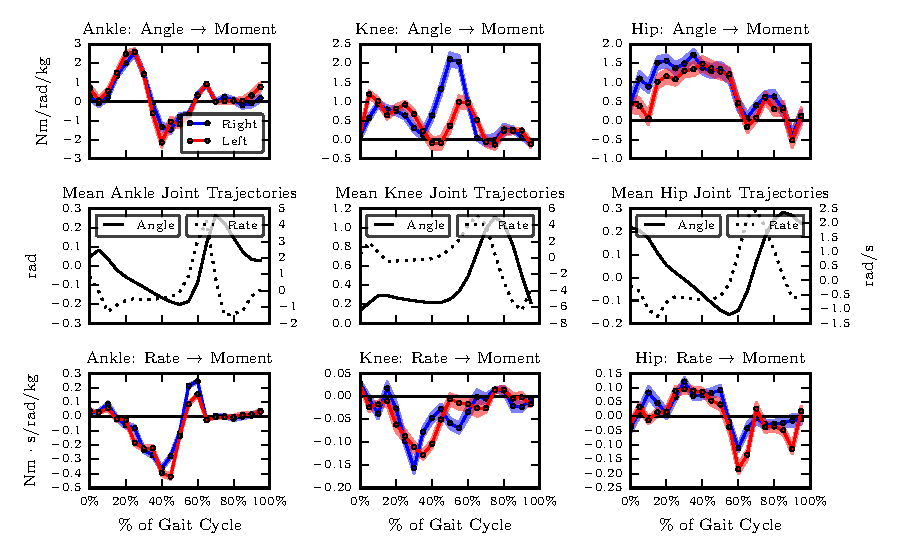
\includegraphics{figures/example-identified-joint-isolated-gains.pdf}
    \caption{Gait phase percent scheduled gains for right (blue) and left (red) legs.}
    \label{fig:example-gains}
  \end{center}
\end{figure}

Here we present an example result from a controller structure which is limited
to joint torque generation only from error in the sensors from the same joint.
Figure \ref{fig:gains} shows the estimates of the scheduled gains with respect
to the percent gait cycle in each leg. Figure \ref{fig:fit} demonstrates an
example prediction of the measured ankle plantarflexion torque in the right leg
by the identified control model.
%
%\begin{figure}[b]
  %\begin{center}
    %\includegraphics[width=\columnwidth]{fig/fit.pdf}
    %\caption{Predicted torque compared to independent validation data.}
    %\label{fig:fit}
  %\end{center}
%\end{figure}
%
\subsection*{$\mathbf{m}^*$ accounts for most of the variation}
%
\subsection*{Random variations predict random gains}
%
\subsection*{Similar gains are predicted from both unperturbed and perturbed}
%
\subsection*{Increasing the number of sensors for each control increases vaf}
\section*{Discussion}
%
We are able to identify a simple linear controller that exhibits larger gains
in the stance phase than in the swing phase. Additionally, similar gain
patterns in the right and left legs are observed that use both positive and
negative feedback. The controller is capable of predicting the measured joint
torques with greater than 65\% VAF in all joints. Results and conclusions from
a larger sample of subjects and conditions will be presented at the conference.

%\section*{Acknowledgments}
%
%This research was funded by the Ohio's Wright Center for Sensor Systems
%Engineering and the Parker Hannifin Corporation.

\end{document}
